\documentclass{article}

%\usepackage[margin=3.7cm]{geometry}
\usepackage[utf8]{inputenc} 
\usepackage[T1]{fontenc}
\usepackage[brazil]{babel}
\usepackage{mathtools, amssymb} %{amsmath}
\usepackage{amsmath}
\usepackage{float}
\usepackage{graphicx}
\usepackage{wrapfig}
\usepackage[style=brazilian]{csquotes}
\usepackage[dvipsnames]{xcolor}
\usepackage{complexity}
\usepackage{diagbox}
\usepackage{amsfonts}
\usepackage{algorithm,algpseudocode}
\usepackage{hyperref}



% TODO: Apagar
\usepackage[colorinlistoftodos, color=yellow]{todonotes}

\setlength{\parskip}{1em} %espaço entre os parágrafos%

\graphicspath{ {Imagens/} }

\newenvironment{algoritmo}[1][]
  {\begin{algorithm}[#1]
     \selectlanguage{brazil}%
     \floatname{algorithm}{Algoritmo}%
  }
  {\end{algorithm}}

\algnewcommand{\algorithmicand}{\textbf{ and }}
\algnewcommand{\algorithmicor}{\textbf{ or }}
\newcommand{\algorithmicbreak}{\textbf{break}}
\algnewcommand{\OR}{\algorithmicor}
\algnewcommand{\AND}{\algorithmicand}
\newcommand{\BREAK}{\State \algorithmicbreak}

\begin{document}
	\begin{wrapfigure}{L}{0.3\textwidth}
		\begin{flushleft}	
			
\includegraphics[height=.065\textheight]{PESC.png}
		\end{flushleft}
	\end{wrapfigure}

	\quad\\
	{Universidade Federal do Rio de Janeiro} \\
	{Otimização Combinatória - COS890} \\
	{Professor: Abilio Lucena}
	
	\quad\\
	\vspace*{2cm}
	
	\begin{center}
		\huge\bfseries
		Leilões Combinatórios - uma aplicação do problema de empacotamento de conjuntos através de métodos exatos
	\end{center}
	\vspace*{3mm}
	
	\begin{center}
		\large
		Amanda Camacho Novaes de Oliveira
		
		Diego Amaro Ferraz da Costa	
		
		Diego Athayde Monteiro 
	\end{center}

	\vspace{1cm}
	
	
	\begin{abstract}
	    Neste trabalho, descrevemos o problema dos leilões combinatórios como uma aplicação do \textsc{Problema de Empacotamento de Conjuntos}, primeiramente proposto por Karp \cite{Karp}. Aplicamos três algoritmos exatos para a resolução do mesmo: \textbf{Relaxação Lagrangeana}, \textbf{Branch-and-Bound} e \textbf{Branch-and-Cut}. Os mesmos foram implementados através do solver \emph{Gurobi}, utilizando a linguagem de programação \emph{Julia} e biblioteca \emph{JuMP}. Utilizamos diferentes instâncias para comparar o desempenho dos algoritmos, obtendo ... \todo{Colocar algum resultado de interesse} 
	\end{abstract}
	\newpage
	
	
	\section{Introdução}
	A otimização combinatória é a área que estuda problemas de otimização aplicados a conjuntos discretos. Os problemas de otimização são aqueles onde se procura determinar valores extremos de um conjunto de restrições, com respeito a uma função, esta chamada de função objetivo. As variáveis envolvidas nos problemas de otimização são denominadas variáveis de decisão. Pode-se classificar os problemas de otimização combinatória de acordo com os tipos de variáveis que os compõem: variáveis lineares ou não lineares; variáveis binárias, inteiras ou reais.
	%Quando falamos destas variáveis, podemos dividir os problemas de otimização em duas categorias: problemas onde as variáveis são lineares e problemas onde elas são não-lineares. E ainda podemos fazer mais uma distinção quanto aos problemas de otimização combinatória que estamos lidando, e esta distinção é através dos valores que as variáveis podem assumir. Podemos ter problemas onde as variáveis podem assumir valores reais, inteiros, binários ou ainda um misto destas classificações.
	
	Neste trabalho, definimos e aplicamos técnicas de soluções exatas para um conhecido problema, o \textsc{Problema de Empacotamento de Conjuntos (PEC)}.
	% Mais especificamente, sua versão de otimização.
	Ele consiste em encontrar uma combinação de subconjuntos de elementos de forma que se obtenha peso máximo e que nenhum elemento seja selecionado por mais de um conjunto. Pode ser descrito como um problema de programação inteira onde as variáveis são lineares e podem assumir valores binários 0-1.
	%: dado um cojunto finito $I$ de $n$ elementos e um conjunto finito $J$ de $m$ elementos, desejamos obter o conjunto $I_j$ dos subcojuntos viáveis (a cada um destes subconjuntos é associado um peso $c_j$) de $I$ com o maior peso possível. Vamos definir de maneira mais formal, detalhar o problema e sua formulação em uma seção mais adiante.
	
	Este problema possui muita aplicação prática e uma das mais conhecidas é a de Leilões Combinatórias que é abordagem que fazemos neste trabalho. Um leilão combinatório consiste em distribuir um número $m$ de produtos através de $n$ lances. Se um lance é escolhido, um determinado lucro é obtido. O objetivo em um leilão combinatório é maximizar o lucro total respeitando a condição de que cada produto só pode estar contido em no máximo um lance. Utilizando esta aplicação do PEC, utilizamos três métodos exatos para resolver o problema: uma \textbf{Relaxação Lagrangeana}, um algoritmo \emph{\textbf{Branch-and-Bound}} e um segundo algoritmo \emph{\textbf{Branch-and-Bound}} com algoritmos de planos de corte associados ao mesmo, denominado \emph{\textbf{Branch-and-Cut}}.
	
	Esse texto está organizado da seguinte forma: na seção~\ref{sec:prob}, detalhamos o \textsc{Problema de Empacotamento de Conjuntos}, e nas seções \ref{sec:relag}, \ref{sec:BB} e~\ref{sec:BC} descrevemos um pouco cada método aplicado. Nas seções~\ref{sec:res} e~\ref{sec:disc} exibimos os resultados obtidos e a comparação entre os métodos e, por fim, na seção~\ref{sec:concl} nossas conclusões e ideias para trabalhos futuros.
	
	
	\section{O Problema de Empacotamento de Conjuntos}\label{sec:prob}
	O \textsc{problema de empacotamento de conjuntos} (PEC) (do inglês, \emph{Set-Packing Problem}) foi um dos 21 problemas enunciados por Karp em \cite{Karp}. Neste mesmo trabalho, Karp mostrou que se trata de um problema \NP-completo através de uma redução feita do problema da clique máxima de um grafo. O PEC também possui forte relação com o problema da cobertura de conjuntos, estes formando um par dual-forte.
	
	O PEC pode ser descrito pelo ponto de vista da decisão, que consiste em determinar, dado um inteiro $k$, se existe um conjunto com $k$ subconjuntos do conjunto de subconjuntos viáveis $I_j$.
	Porém neste trabalho abordamos a versão de otimização, cuja descrição formal é dada da seguinte forma:
	
	\begin{itemize}
	    \item[-] $I$ = \{1, ..., m\}: conjunto finito de elementos
	    
	    \item[-] $J$ = \{1, ..., n\}: conjunto finito de índices
	    
	    \item[-] \{$I_j$ $\subseteq$ : $j$ $\in$ $J$\}: conjuntos dos subconjuntos viáveis de $I$
	    
	    \item[-] Existe um peso $c_j$ à cada $I_j$, $j$ $\in$ $J$
	    \{$I_j$ $\subseteq$ : $j$ $\in$ $J$\}: conjuntos dos subconjuntos viáveis de $I$
	    
	    \item[-] \{$I_j$ : $j$ $\in$ $J_i$\}: subconjuntos dos subconjuntos viáveis de $I$ que contém $i$~$\in$~$I$
	    \item[-] Variáveis binárias $x_j$ $\in$ \{0,1\} que expressam a decisão de escolher ou não $I_j$, $j$~$\in$~$J$
	\end{itemize}
	
	
	Dadas estas definições, sua formulação como um problema de programação inteira está dada pela equação \ref{eq:PEC-prof}.
	
	\begin{equation}
		\label{eq:PEC-prof}
        \begin{array}{ll@{}ll}
            \text{max}  & \displaystyle\sum\limits_{j \in J} c_{j}&x_{j} &\\
            \text{sujeito a}& \displaystyle\sum\limits_{j \in J_i}   &x_{j} \leq 1,  &i \in I\\
                 &                                                &x_{j} \in \{0,1\}, &j \in J
        \end{array}
    \end{equation}
    
	Este problema possui uma ampla aplicação prática. Como um exemplo destas, temos o escalonamento de tripulações de companhias aéreas para aviões. Cada avião da frota precisa ter uma tripulação designada a ele, composta por um piloto, copiloto e navegador~\cite{Airline}.    
    Como mencionado anteriormente, a abordagem que fazemos aqui ao \textsc{problema de empacotamento de conjuntos} é feita no contexto dos leilões combinatórios, que é objeto de estudo de muitos estudiosos em diversos trabalhos (\cite{Winner}, \cite{Taming}, \cite{CABOB}). Nesta aplicação os conjuntos $I$ e $J$ podem ser enxergados como um conjunto de $m$ produtos e um conjunto de $n$ lances, respectivamente. Nosso objetivo então é maximizar o lucro total obtido sem violar a restrição de que um produto só pode ser escolhido por, no máximo, um lance. E este lucro é um valor associado a seleção de cada lance. 
    Para a solução desse problema implementamos uma formulação alternativa, dada pela equação \ref{eq:PEC}, onde $ a_{ij} $ vale $ 1 $ se o lance $ j $ seleciona o produto $ i $, ou $ 0 $ caso contrário.
    
    \begin{equation}
    	\label{eq:PEC}
    	\begin{array}{ll@{}ll}
    		\text{max}  & \displaystyle\sum\limits_{j = 0}^{n} c_{j} & x_{j} &\\
    		\text{sujeito a}& \displaystyle\sum\limits_{j = 0}^{n}   & a_{ij}x_{j} \leq 1,  & i=1,\cdots,m\\
    		&                                                &x_{j} \in \{0,1\}, & j = 1,\cdots,n
    	\end{array}
    \end{equation}
    
    Esta formulação, também observada em outros trabalhos como \cite{guo2005using}, por exemplo, foi utilizada por entendermos que ela é mais intuitiva, sendo mais fácil de vizualizar e entender o problema dessa forma. Entretanto, foi observado ao longo da implementação que a formulação dada pela equação \ref{eq:PEC-prof} é mais eficiente para instâncias muito grandes, uma vez que na maioria dos casos as matrizes $ A $ induzidas pela seleção de produtos por lances são esparsas. 
	
	
	\section{Relaxação Lagrangeana}\label{sec:relag}
	A relaxação lagrangeana consiste em um método de decomposição das restrições de um determinado problema em dois grupos: as restrições \enquote{convenientes} e as restrições \enquote{inconvenientes}. 
	Chamamos de restrições \enquote{inconvenientes} aquelas que fazem com que o problema se torne difícil de resolver. Dessa forma tais restrições são
	retiradas do problema de programação inteira e adicionadas à função objetivo em um termo $u(d - Dx)$. Estas variáveis $u_i$ são denominadas variáveis duais ou multiplicadores de Lagrange.
	
	Nem sempre a relaxação lagrangeana nos oferece uma solução ótima para o problema. Ela é limitada pelos resultados da relaxação linear. O segundo grupo de restrições, as \enquote{convenientes} tornam o problema mais fácil de ser resolvido e eventualmente podemos obter a solução ótima para o problema original através da relaxação.
	
	O ponto de partida para a aplicação deste método é a elaboração do subproblema lagrangeano. Baseado no modelo de programação inteira que apresentamos na seção~\ref{sec:prob}, o subproblema lagrangeano para o PEC é: 
	
	\begin{equation*}
        \begin{array}{ll@{}ll}
            \text{max}  & \displaystyle\sum\limits_{j \in J} (c_{j} - \displaystyle\sum\limits_{i \in I_j} u_{j})x_j+  \displaystyle\sum\limits_{i \in I} u_{i}\\
            \text{sujeito a}
                 &                                                x_{j} \in \{0,1\}, j \in J
        \end{array}
    \end{equation*}
	
	% \begin{algorithm}
    %     \caption{Subgradiente para o problema de empacotamento de conjuntos}
    %     \begin{algorithmic}[1]
    %         %\Statex \textbullet~\textbf{Parameters:} $n, t \in % \mathbb{N}$, where $t < n$.
    %         \State \For{$k = 0$, $k < $maxInt, $ k++$}
    %         \State $z_u$, $x_u$ = limite\_superior()
    %         \State $z_l$, $x_l$ = limite\_inferior()
    %         
    %         
    %         \State Second step
    %         \State \ldots
    %     \end{algorithmic}
    % \end{algorithm} 
	
	O algoritmo abaixo em conjunto com uma heurística gulosa para obtenção de limites inferiores resumem a abordagem adotada para o PEC utilizando o método da relaxação Lagrangeana. A obtenção de limites inferiores consiste em ordenar o conjunto de lances e e selecionar o que apresenta o maior valor calculado pela razão do custo lagrangeano daquele lance em questão pelo número de produtos que o lance cobre. Os resultados obtidos serão exibidos na seção~\ref{sec:res}.
	
	\begin{algoritmo}[H]
    \caption{Subgradiente para o problema de empacotamento de conjuntos}
        \begin{algorithmic}[1]
            \Statex {\color{gray}\it Variáveis:}
            \State MaxIter $=$ Número máximo de iterações definido
            
            \State s = zeros(m), sqrSum = 0, $\pi_{min}$ = 0.0001
            
            \State $k = 0$ \Comment{{\color{gray}\it Índice da iteração}}
            
            \Statex
            \Statex {\color{gray}\it Começar loop}
            \State Definir $\pi = 2$ e multiplicadores de Lagrange $u = 0$
            
            \State \textbf{while} $k<$ MaxIter \textbf{then}
            
            \State \indent Resolver o subproblema Lagrangeano, obtendo: $\overline{x}$, $\overline{z}$
            
            \State \indent Encontrar soluções viáveis a partir da solução relaxada: $\underline{x}$, $\underline{z}$
            
            \State \indent $k = k + 1$
            
            \Statex
            \Statex \qquad {\color{gray}\it Critérios de Parada:}
            
            \State \indent \textbf{if} {$k \equiv $ MaxIter \OR $\pi < \pi_{min}$} \textbf{then}   
            \State \indent \indent \Return $ \underline{x} $
            \Statex
            %\State \EndIf
            \State \indent \textbf{if} $( \overline{z} - \underline{z} < 1 )$ \OR ($\underline{x}$ é viável e a função de otimização tem mesmo valor tanto na versão primal quanto na dual para os multiplicadores $u$ e a solução $\underline{x}$)   \textbf{then}
            \State \indent \indent \Return \underline{x} \Comment{{\color{gray}\it Encontrado o valor ótimo}}
            %\State \EndIf
            
            \Statex
            \Statex \qquad {\color{gray}\it Atualização de $\pi$}
            \State \indent \textbf{if} {{$\dfrac{\lfloor{MaxIter}\rfloor}{20}$} iterações consecutivas sem melhora} \textbf{then} 
            \State \indent \indent $\pi := \pi/2$
            %\State \EndIf
            %\State \EndIf
            %\underline{}
            
    
            \Statex
            \Statex \qquad {\color{gray}\it Atualização dos multiplicadores de Lagrange: }
            \State \indent \textbf{for}{ cada produto $i$} \textbf{do}
            \State \indent \indent $s[i] = 1 - \sum_{j\in L} a[i,j]*\overline{x}[j]$
            \State \indent \indent $u_i = \max \{0,(1+ \epsilon) T \cdot s_i\}, \quad \forall i= 1,\dots,m$
            \State \indent \indent sqrSum = sqrSum + $s[i]^2$
            %\Statex
            \State \indent$T = \dfrac{\pi * (\overline{z} - \underline{z})}{\text{sqrSum}} $
            %\Statex
            \State \indent \textbf{if}{ $T < \pi_{min}$}\textbf{ then}
            \State \indent \indent \Return $\underline{x}$ \Comment{{\color{gray}\it Parada por valor muito pequeno do passo}}
            %\State \EndIf
            %\Statex
            \State \indent \textbf{for} { cada produto $i$} \textbf{do}
            \State \indent \indent $u[i] = max(0, u[i] - T*s[i]) $
            %\State \EndFor
            %\Statex
            %\State Retornar para a linha 5
        \end{algorithmic}
    \end{algoritmo}

	
	\section{Branch and Bound}\label{sec:BB}
	Uma técnica muito aplicada para resolução de problemas combinatórios é a técnica de dividir e conquistar que consiste em resolver subproblemas mais fáceis que o original e após este processo combinar as soluções obtidas até obtermos a solução do problema original. Porém, esta enumeração de subproblemas de forma explícita pode ser muito custosa, e justamente neste contexto, é que algoritmo \emph{Branch-and-Bound} entra em ação.
	
	O algoritmo \emph{Branch-and-Bound} consiste em uma técnica de enumeração implícita de soluções, onde através de limites locais, obtemos limites globais. Toda a eficiência e ganho que o algoritmo \emph{Branch-and-Bound} nos oferece é por conta das podas que acontecem na árvore de enumeração implícita, que podem ocorrer por: otimalidade, inviabilidade e limites duais. A técnica foi definida primeiramente em~\cite{Land} por Ailsa Land e Alison Doig em 1960, e figura como um dos mais importantes métodos exatos no contexto de resolução de problemas de otimização até os dias atuais.
	
	
	Para a implementação do método \emph{Branch-and-Bound}, fizemos uso de uma abordagem mais direta, onde o próprio solver já executa o método por padrão. Foram desabilitadas funções como cortes, múltiplas threads, métodos de pré-processamento e afins. Isto foi feito para termos uma noção mais exata do comportamento do método. A partir desta forma de resolver o problema, extraímos algumas informações importantes como: número de nós explorados pela árvore de enumeração e tempo de excução.
	
	
	
	\section{Branch and Cut}\label{sec:BC}
	Para fortalecermos ainda mais o algoritmo \emph{Branch-and-Bound}, é possível utilizarmos de algoritmos de planos de corte em cada nó de sua árvore de enumeração. Dessa forma pode-se fortalecer a formulação do problema através da adição de informações adicionais antes de efetuar o \emph{Branching} de um determinado nó. Isso faz com que se gaste mais tempo em cada nó, na esperança de que isso diminua o número de nós explorados e o tempo total de utilização da CPU.
	
	Como desigualdades válidas para o PEC, utilizamos desigualdades de cliques geradas a partir de um grafo conflito. Este grafo é definido da seguinte forma: cada lance no problema de leilões combinatórios define um vértice do grafo,
	e dois vértices possuem aresta entre si se ambos os lances selecionam um mesmo produto. Como quaisquer lances conectados selecionam pelo menos um produto em comum, no máximo um lance de cada clique pode ser selecionado para uma solução viável.
	

	%\begin{algoritmo}[H]
    %\caption{Branch and Cut}
     %   \begin{algorithmic}[1]
      %      \Statex Variáveis:
       %     \State vizinhos = Array[]
        %    \Statex Definindo vizinhanças:
         %   \State \For{j em Lances}
          %  \State viz = Array[]
           % \State \For{i em Produtos}
            %\State \If{$a[i,j] \equiv 1$}
            %\State \If{$sum(a[i,:]) > 1$}
            %\State \For{$j_2$ em Lances}
            %\State \If{$a[i,j_2] \equiv 1 \AND j_2 \neq j \AND j_2 %\notin viz $}
            %\State Adiciona $j_2$ no Array $viz$
            %\State \EndIf
            %\State \EndFor
            %\State \EndIf
            %\State \EndIf
            %\State \EndFor
            %\State \EndFor
            
        %\algstore{branchandcut}
        %\end{algorithmic}
    %\end{algoritmo}
    
    O algoritmo abaixo é resultante da estratégia descrita no parágrafo anterior. Utilizando o algoritmo de Bron-Kerbosch~\cite{Bron1973}, enumeramos todas as cliques maximais do grafo de conflito e as adicionanos como desigualdades válidas fortes. Utilizando-se desse método, conseguimos diminuir bruscamente o número e nós explorados na árvore de enumeração implícita em diversos casos.
    
    
    \begin{algoritmo}[H]
    \caption{Branch and Cut}
        \begin{algorithmic}[1]
            \Statex {\color{gray}\it Variáveis:}
            \State vizinhos = Array[]
            \Statex {\color{gray}\it Definindo vizinhanças:}
            \State \textbf{for}{ j em Lances } \textbf{do}
            \State \indent viz = Array[]
            \State \indent \textbf{for}{ i em Produtos } \textbf{do}
            \State \indent \indent \textbf{if}{ $a[i,j] \equiv 1$ } \textbf{then}
            \State \indent \indent \indent \textbf{if}{ $sum(a[i,:]) > 1$ }\textbf{then}
            \State \indent \indent \indent \indent \textbf{for}{ $j_2$ em Lances } \textbf{do}
            \State \indent \indent \indent \indent \indent \textbf{if}{$a[i,j_2] \equiv 1 \AND j_2 \neq j \AND j_2 \notin viz $} \textbf{then}
            \State \indent \indent \indent \indent \indent \indent Adiciona $j_2$ no Array $viz$
            %\State \EndIf
            %\State \EndFor
            %\State \EndIf
            %\State \EndIf
            %\State \EndFor
            %\State \EndFor
            \Statex
            \Statex {\color{gray}\it Algoritmo de Bron-Kerbosch} 
            \State \textbf{function}\textsc{ acharclique}(clique, candidatos, excluidos, output) 
            \State \indent \textbf{if}{ candidatos \AND excluidos sejam vazios }\textbf{then}
            \State \indent \indent Adiciona clique em output
            \State \indent \textbf{for}{ $v \in $ candidatos }\textbf{do}
            \State \indent \indent $R_2 = \text{clique} \cup \{v\}$
            \State \indent \indent $P_2 = \text{candidatos} \cap \text{vizinhos}[v]$
            \State \indent \indent $X_2 = \text{excluidos} \cap \text{vizinhos}[v]$
            \State \indent \indent \textsc{acharclique}($R_2, P_2, X_2, \text{output}$)
            \State \indent \indent candidatos $=$ candidatos $ \backslash ~ \{v\}$
            \State \indent \indent excluidos $=$ excluidos $\cup ~ \{v\}$
            \Statex
            \Statex {\color{gray}\it Algoritmo de Corte}
            \State \textbf{function}\textsc{ CORTE}()
            \State \indent $eps = 0.0001$
            \State \indent Pega um novo nó
            \State \indent \textbf{if}{ $status \equiv valor\_otimo$  }\textbf{then}
            \State \indent $x\_val = valores\_instancia$ 
            \State \indent \textbf{for}{ $clique \in output$}
            \State \indent \indent $soma = 0$
            \State \indent \indent \textbf{for}{ $j \in clique$}
            \State \indent \indent \indent $soma = soma + x\_val[j]$
            \State \indent \indent \textbf{if}{ $soma > 1 + eps $ }\textbf{then}
            \State \indent \indent \indent {\color{gray}\it Restrição violada pela clique}
            \State \indent \indent \indent $valores = $ Array tamanho de todas cliques encontradas
            \State \indent \indent \indent Efetuar corte $\forall clique < 1.0+eps$ (violação da restrição)
            \State \indent \indent \indent $valores = $ Cliques que violaram o corte
            \State \indent \textbf{ return }{valores}
            
            \State 
        \end{algorithmic}
    \end{algoritmo}
	
	\section{Resultados}\label{sec:res}

	Ao longo desta seção são comparados os resultados obtidos pelos três métodos implementados -- Relaxação Lagrangeana, \emph{Branch-and-Bound} e \emph{Branch-and-Cut} -- aplicados a diferentes instâncias do problema de leilões combinatórios.
	
	Inicialmente os três foram aplicados a um caso base simples, de 3 produtos e 4 lances, apenas para verificar o funcionamento correto das implementações. Em seguida aplicamos os mesmo algoritmos em casos maiores, com o objetivo de avaliar o valor ótimo encontrado para essas instâncias. 
	
	Abaixo detalharemos, as informações relevantes, para cada instância utilizada, considerando os resultados obtidos em cada um dos algoritmos executados.
	
		\subsection{Caso Base} \label{sec:caso}
	    Para fins comparativos com os métodos que foram aplicados para a resolução do \textsc{problema de empacotamento de conjuntos}, utilizamos como instância de teste a chamada \textit{toy2}, com 3 produtos e 4 lances, que pode ser observada na tabela \ref{tab:toy2}.
	    
	    \begin{table}[h]
	        \centering
	        \begin{tabular}{|c|c|c|c|c|}
	            \hline
	            \backslashbox{\bf Produto}{\bf Lance} & $ l_1 $ & $ l_2 $ & $ l_3 $ & $ l_4 $ \\\hline
	            $ p_1 $ & 1 & & 1 & \\\hline
	            $ p_2 $ & & 1 & & 1\\\hline
	            $ p_3 $ & & & 1 & 1 \\\hline
	            \multicolumn{5}{c}{\quad} \\\hline
	            \textbf{Valor do lance} & 10 & 12 & 18 & 22 \\\hline
	        \end{tabular}
	        \caption{Instância de teste \textit{toy2}. Na tabela principal, a ocorrência de um valor $1$ entre o lance $l_j$ e o produto $p_i$ significa que $p_i$ é selecionado por $l_j$.
	        A linha de valores especifica o ganho que a seleção de cada lance $l_j$ trás.}
	        \label{tab:toy2}
	    \end{table}
	    
	    Esta é uma instância muito simples, criada especificamente para testar o funcionamento adequado dos métodos. É esperado que, para este caso, todos os métodos sempre encontrem o valor ótimo e que nenhum apresente problemas para chegar a essa solução. Neste exemplo, o valor ótimo é $32$, obtido quando se seleciona os lances 1 e 4.
	    %As observações práticas corresponderam às espectativas. 
	    
	    Na prática, todos os três métodos foram capazes de encontrar o valor ótimo. A relaxação lagrangeana o fez em 63 iterações, enquanto o \emph{Branch-and-Bound} e o \emph{Branch-and-Cut} encontraram a solução em 1 iteração simplex. Todos resolvem em menos de $10$~ms.
	    
	    Como o problema é muito simples de resolver, ele não foi o suficiente para averiguar as vantagens do algoritmo \emph{Branch-and-Cut}. Isso será feito com instâncias mais complexas que serão vistas ao longo desta seção.
	    
	    % utilizamos como principal a instância abaixo extraída de~\cite{Elisa}:
	    % \begin{figure}[H]
        %     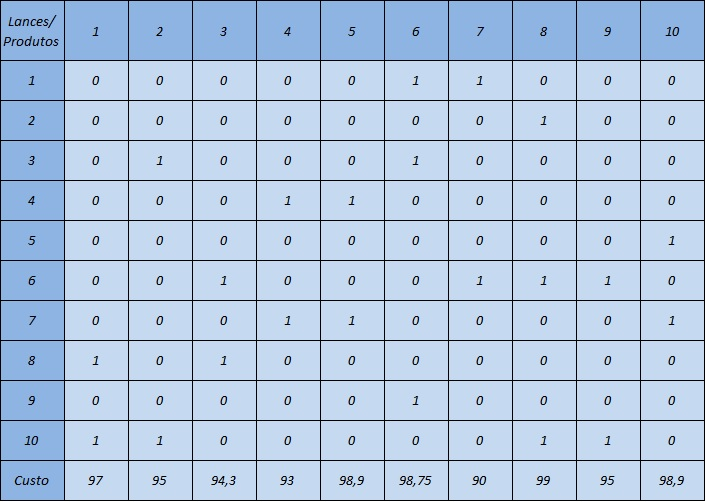
\includegraphics[scale=0.65]{Imagens/Tabela.jpg}
        %     \centering
        %     \caption{Instância}
        % \label{fig:instance}
        % \end{figure} 
	    %\todo[inline]{Descrever como é a tabela}
	    
	    
    \subsection{Leilão de energia elétrica (10 x 10)}
    
    Este é um exemplo baseado no cenário de geração de energia elétrica adaptado de \cite{Elisa}. Foi extraída uma relação de 10 produtos e 10 lances, a qual pode ser observada na tabela \ref{tab:inst10}.
    
    \begin{table}[h]
	    \centering
        \resizebox{\textwidth}{!}{
	    \begin{tabular}{|c|c|c|c|c|c|c|c|c|c|c|}
	        \hline
	        \backslashbox{\bf Produto}{\bf Lance} & $ l_1 $ & $ l_2 $ & $ l_3 $ & $ l_4 $ & $ l_5 $ & $ l_6 $ & $ l_7 $ & $ l_8 $ & $ l_9 $ & $ l_{10} $ \\\hline
	        $ p_1 $ & & & & & & 1 & 1 & & & \\\hline
	        $ p_2 $ & & & & & & & & 1 & & \\\hline
	        $ p_3 $ & & 1 & & & & 1 & & & & \\\hline
	        $ p_4 $ & & & & 1 & 1 & & & & & \\\hline
	        $ p_5 $ & & & & & & & & & & 1 \\\hline
	        $ p_6 $ & & & 1 & & & & 1 & 1 & 1 & \\\hline
	        $ p_7 $ & & & & 1 & 1 & & & & & 1 \\\hline
	        $ p_8 $ & 1 & & 1 & & & & & & & \\\hline
	        $ p_9 $ & & & & & & 1 & & & & \\\hline
	        $ p_{10} $ & 1 & 1 & & & & & & 1 & 1 & \\\hline
	        \multicolumn{10}{c}{\quad} \\\hline
	        \textbf{Valor do lance} & 97.00 & 95.00 & 94.30 & 93.00 & 98.90 & 98.75 & 90.00 & 99.00 & 95.00 & 98.90 \\\hline
	   \end{tabular}
	   }
	   \caption{Leilão de energia elétrica. Na tabela principal, a ocorrência de um valor $1$ entre o lance $l_j$ e o produto $p_i$ significa que $p_i$ é selecionado por $l_j$.
	   A linha de valores especifica o ganho que a seleção de cada lance $l_j$ trás.}
        \label{tab:inst10}
    \end{table}
    
    Este exemplo tem solução ótima com lucro de $ 296{,}65 $, obtido através da seleção dos lances $ l_6 $, $ l_8 $ e $ l_{10} $. Tal resultado foi alcançado pelas técnicas \emph{Branch-and-Bound} e \emph{Branch-and-Cut}. A relaxação lagrangeana, no melhor caso, chegou no valor $ 290{,}75 $ ao rodar o algoritmo por $1.000$ iterações. O algoritmo levou $0{,}20$~s para terminar.
    
    Uma análise mais profunda mostrou que neste caso o algoritmo da relaxação lagrangeana não consegue solução melhor porque o limitante superior, por ela obtido está limitado pelo valor da relaxação linear, independente da quantidade de iterações executadas no algoritmo, que neste caso é $ 342{,}8 $ (obteve-se $ 342{,}83 $ para o melhor limitante superior por relaxação lagrangeana). É interessante observar que existe uma grande diferença entre o resultado ótimo do problema com variáveis binárias e de sua relaxação linear, mesmo sendo essa uma instância relativamente pequena. 
    
    \begin{table}[h]
	        \centering
	        \resizebox{\textwidth}{!}{
	        \begin{tabular}{|c|c|c|c|c|c|c|}
	            \cline{2-7}
	            \multicolumn{1}{c|}{ } &  \multicolumn{2}{c|}{Relaxação Lagrangeana} & \multicolumn{2}{c|}{Branch \& Bound} & \multicolumn{2}{c|}{Branch \& Cut}\\\hline
	            \multicolumn{1}{|c|}{ } & Melhor Solução &  Tempo Execução & Nós explorados &  Tempo Execução & Nós explorados &  Tempo Execução \\\hline
	            Caso base & & & & & &  \\\hline
	            Leilões (10x10) & $ 290{,}75 $ & $0{,}1998$ & $7$ & $0{,}02$ & $3$ & $0{,}01$ \\\hline
	            Benchmark (500x100) - PV & $347{,}00$ & $0{,}41$ & $1036$ & $0{,}51$ & $95$ & $0{,}31$ \\\hline
	            Benchmark (500x100) - PU & $32{,}00$ & $0{,}26$ & $1148$ & $0{,}31$ & $35$ & $0{,}14$ \\\hline
	            %Branch \& Bound & $ 296{,}65 $ & $0{,}02$\\\hline
	            %Branch \& Cut & $ 296{,}65 $ & $0{,}01$ \\\hline
	        \end{tabular}
	        } 
	        \caption{Tempo de execução é calculado em segundos. Escrever aqui...}
	        \label{tab:tempos}
	    \end{table}
    
    Pode-se observar a resolução pelo método \emph{Branch-and-Bound} clássico resultou na análise de 7 nós da árvore induzida, levando um total de $0{,}02$~s, enquanto o \emph{Branch-and-Cut}, com a adição dos planos de corte, só precisou analisar 3 nós para encontrar a solução ótima, durando $0{,}01$~s. 
    
    O grafo de conflito desta instância, apresentado na figura \ref{fig:instance}, apresenta 6 cliques maximais: $\{1, 2, 8, 9\}$, $\{1, 3, 8, 9\}$, $\{2, 6\}$, $\{3, 7, 8, 9\}$, $\{4, 5, 10\}$ e $\{6, 7\}$.
    Durante a execução do algoritmo \emph{Branch-and-Cut} foi aplicando um corte, dado pela clique $\{ 1, 3, 8, 9 \}$, que foi violada na análise de um dos nós do \emph{Branch-and-Bound}.
    
    \begin{figure}[H]
        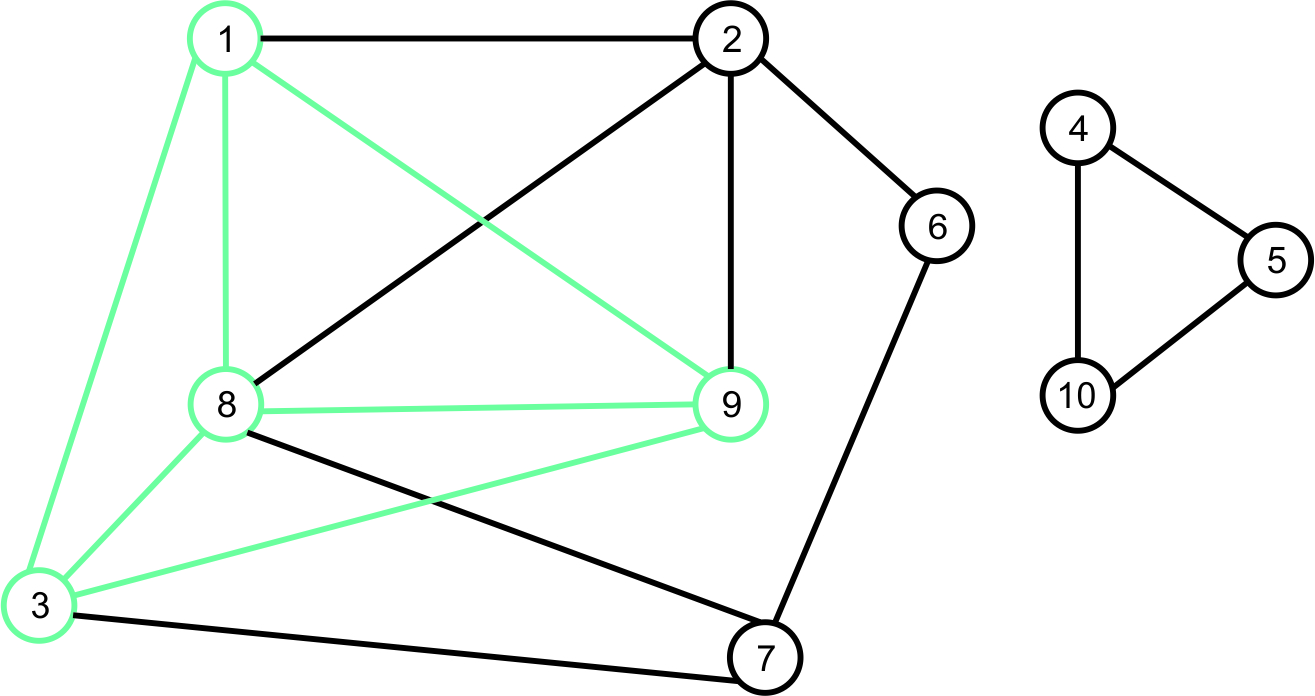
\includegraphics[scale=0.65]{Imagens/GrafoClique.jpg}
             \centering
             \caption{Grafo de conflito do leilão de energia elétrica. Em verde está assinalada a clique aplicada como plano de corte na execução do \emph{Branch-and-Cut}.}
         \label{fig:instance}
    \end{figure} 

    \subsection{Instâncias de referência}
    
    Para analisar melhor as propriedades dos métodos implementados, \todo{Especialmente do Branch-and-Cut?}
    foram selecionadas instâncias do PEC com grande número de produtos e lances. Com muitas variáveis e restrições o problema se torna mais difícil e é necessário um maior esforço por parte dos métodos.
    
    As instâncias aqui utilizadas foram extraídas da fonte \cite{benchmarks}, que contém um conjunto de \emph{Benchmarks} para o PEC. Os resultados para cada uma das instâncias escolhidas pode ser observado a seguir. \todo{Conferir \\ Possivelmente podemos colocar uma tabela com os resultados aqui no geral? Ou talvez nao seja melhor colocar resultados das instâncias antes das próprias instâncias.. Talvez só colocar uma tabela com as características das instâncias escolhidas, parecido com o que tem no site}
    %O primeiro exemplo utilizado, na seção \ref{sec:res:ssec:bchmrk1}, possui valores de lances variados
    
    
    \subsubsection{Benchmark 500 x 100 - Pesos variáveis}% - 2 produtos por lance, Preços variados}
    \label{sec:res:ssec:bchmrk1}
    \todo[inline]{Rever esse título. Provavelmente o que queremos colocar aqui vai depender das outras instâncias que a gente utilizar}
    
    Este primeiro \emph{benchmark} corresponde à instância \enquote{pb\_100rnd0100.dat}, na qual tem-se 500 produtos e 100 lances. Os preços de cada lance são variados, podendo valer de 1 a 20, e cada produto é coberto por dois lances. O valor ótimo dessa instância é $372$.
    
    O \emph{Branch-and-Bound} obteve valor máximo explorando $ 1036 $ nós (em $ 0{,}51 $~s), enquanto o \emph{Branch-and-Cut} a obteve explorando apenas 95 nós ($ 0{,}31 $~s). Foram adicionados 99 planos de corte no \emph{Branch-and-Cut}, o que demonstrou uma clara melhora no desempenho do algoritmo.
    
    A relaxação lagrangeana não converge para o ótimo, o limitante superior convergindo para $ 514{,}5 $. O algoritmo para com aproximadamente $40$~s por estourar o limite de iterações.  Esse resultado, embora não seja o ótimo, fornece o limitante oriundo da relaxação linear, o que é uma informação relavante, e a melhor solução viável encontrada é $347$, o que está relativamente próximo do ótimo de $372$, especialmente quando se considera a grande diferênça com relação ao melhor limitante superior.
    
    
    \subsubsection{Benchmark 500 x 100 - Pesos unitários}
    
    Este segundo \emph{benchmark}, correspondente à instância \enquote{pb\_100rnd0200.dat}, possui as mesmas caracterísitcas que a anterior ($500$ produtos por $100$ lances, 2 lances por produto), com a diferença que os lances têm todos o mesmo peso, no caso um peso unitário. Isso significa que a escolha de um lance trás o mesmo benefício que a escolha de qualquer outro e a seleção de lances ótima vai ser aquela que permitir a escolha do número máximo de lances. O valor ótimo para esta instância é de $34$.
    
    O \emph{Branch-and-Bound} obteve valor máximo explorando 1148 nós, realizando isso em $0{,}31$~s, enquanto o \emph{Branch-and-Cut} explorou apenas 35 nós, tendo aplicado $98$ planos de corte e levando um total de $0{,}14$~s. Ambos os métodos encontraram o valor ótimo, mas pode-se observar um ganho de desempenho qunado se aplica o algoritmo de planos de corte.
    
    Novamente, a relaxação lagrangeana não converge para o ótimo, encontrando o valor máximo de $32$ (ao invés de $34$), com melhor limitante superior equivalente a $50$. O algoritmo rodou por $26$~s e $684$ iterações, quando parou devido por obter um passo de atualização dos multiplicadores de lagrange muito pequeno.
    \todo{O que mais comentar sobre o resultado?}
    
    
    \subsubsection{Benchmark 100 x 100 - Pesos Variáveis}
    \todo[inline]{Verificar se vamos tirar este}
    O terceiro \emph{benchmark} corresponde à instância \enquote{pb\_100rnd0500.dat}, na qual o número de produtos e lances é igual, ambos com cardinalidade 100. A variação ds preços de cada lance está contida na mesma faixa da instãncia anterior, podendo valer de 1 a 20, e cada produto também é coberto por dois lances. O valor ótimo dessa instância é $639$.
    
    %%%%%%%%%%%%%%%%%%%%%%%%%%%%%%%%%%%%%%%%%%%
    
    Entretando, a resolução da instância pelos métodos \emph{Branch-and-Bound} e \emph{Branch-and Cut} se mostrou bem imediata. Ambos realizaram o procedimento em tempo muito pequeno e sem explorar nenhum nó da árvore de enumeração.O \emph{Branch-and-Bound}, mais especificamente obteve valor ótimo de $639$ em $ 0{,}01 $~s, enquanto o \emph{Branch-and-Cut} a obteve em tempo inferior a este. Porém, foram adicionados 31 planos de corte no \emph{Branch-and-Cut} e isto tomou $ 0{,}03 $~s, o que demonstrou um tempo total superior ao do \emph{Branch-and-Bound}, o tornando assim, o método mais eficiente para esta instância.
    
    %%%%%%%%%%%%%%%%%%%%%%%%%%%%%%%%%%%%%%%%%%%
    
    Nesta instância, a relaxação lagrangeana consegue atingir o ótimo, o valor $639$. E encontra este valor em $412$ iterações e leva $ 5{,}073 $~s para fazê-lo.
    
    
    
    \subsection{Instâncias PBP}
    \todo{Trocar título. Descrever instâncias e resultados}
    
    As instâncias avaliadas a seguir foram criadas de acordo com o gerador de conjuntos PBP (\emph{Price Proportional Bid}), descrito em \cite{guo2005using}\footnote{
    Código descrito foi reproduzido no arquivo \enquote{gerador\_pbp.jl}}.
    Os conjuntos de teste PBP geram amostras nas quais o preço de um lance é relacionado à quantidade e qualidade dos produtos que ele cobre, e ao mesmo tempo o preço de um produto é aproximadamente proporcional ao número de lances pelos quais ele é coberto. Isso é um padrão observado em problemas reais de leilões combinatórios que o gerador de conjunto de testes tenta reproduzir.
    
    \todo[inline]{Especificar quais instâncias vão ser usadas...?}
    
    
    \subsubsection{PBP 100 x 50 - Densidade 0,1}
    
    Nesta instância é apresentado um caso com 100 produtos e 50 lances, com densidade de $0{,}1$. O parâmetro de densidade diz respeito à probabilidade de um produto ser coberto por um determinado lance (ou, similarmente, de um lance cobrir um produto). A instância gerada foi chamada \enquote{pbp\_100-50\_dens0.100000.txt}.
    
    Ambos o \emph{Branch-and-Bound} e o \emph{Branch-and-Cut} foram capazes de encontrar o valor ótimo de $285{,}811$. O \emph{Branch-and-Bound} encontrou a solução explorando $79$ nós, e durou em torno de $0{,}06$~s. 
    
    Nesta instância observou-se que a adição do algoritmo de planos de corte não gerou ganho no algortimo de otimização. Pelo contrário, embora acabe explorando apenas $18$ nós, ele levou $2{,}41$~s para rodar, sendo aproximadamente 40 vezes mais lento. Isso ocorre porque há a adição de planos de corte demais para a magnitude do problema, um total de 382 plaos. Esta instância demonstra que possivelmente seria vantajoso para este problema alterar o algoritmo de planos de corte de forma que o mesmo adicione apenas a restrição mais violada ao invés de todas as restrições violadas toda vez que o mesmo é chamado.
    
    
    
    \todo[inline]{Caso 1: pbp_100-50_dens0.100000.txt
    
    BB:
    
    Explored 79 nodes (1137 simplex iterations) in 0.07 seconds
Thread count was 1 (of 4 available processors)

Solution count 4: 285.811 280.434 247.246 245.045 

Optimal solution found (tolerance 1.00e-04)
Best objective 2.858113017420e+02, best bound 2.858113017420e+02, gap 0.0000\%

Segunda vez: 0.04 seconds


—————————

RL:

(256.9960733636211, [0.0, 0.0, 0.0, 0.0, 0.0, 0.0, 0.0, 1.0, 0.0, 0.0  …  0.0, 0.0, 0.0, 0.0, 0.0, 0.0, 0.0, 0.0, 0.0, 0.0])

k_best: 965
Novo z\_up: 421.5758728771783
6.552909452


—————————

BC:

Cutting planes:
  User: 382

Explored 18 nodes (783 simplex iterations) in 2.41 seconds
Thread count was 4 (of 4 available processors)

Solution count 2: 285.811 280.434 

Optimal solution found (tolerance 1.00e-04)
Best objective 2.858113017420e+02, best bound 2.858113017420e+02, gap 0.0000\%

User-callback calls 92, time in user-callback 2.42 sec
    
    }
    
    \todo[inline]{Nota: Embora o BC apresente menor tempo do algorimto de otimizacao em si, nos casos apresentados, em diversas instâncias o tempo que leva para calcular os cliques do diagrama de conflito nao compensa...}
    
	\section{Conclusão}\label{sec:concl}
	Neste trabalho, abordamos o \textsc{problema de empacotamento de conjuntos} e uma aplicação bem conhecida que são os leliões combinatórios. Resolvemos o problema pelo solver \emph{Gurobi}, a linguagem \emph{Julia} e a biblioteca \emph{JuMP} utilizando três métodos exatos e comparamos os resultados obtidos entre eles. Foram usadas diversos tipos de instâncias: algumas de elaboração própria, uma instância extraída de~\cite{Elisa} e outras retiradas de~\cite{benchmarks}. Observamos que a relaxação lagrangeana nem sempre obtinha o valor ótimo, porém em diversos casos obtemos soluções bem próximas do ótimo. Os métodos \emph{Branch-and-Bound} e \emph{Branch-and-Cut} obtiveram as soluções ótimas em todas as instâncias testadas, de maneira que o segundo se mostrou bem mais eficiente em termos de tempo computacional que o primeiro por conta das desigualdades válidas fortes que extraímos a partir de um grafo conflito elaborado com base na instância em questão.
	
	Como trabalhos futuros, pretendemos refinar os métodos implementados para obter soluções mais próximas da solução ótima nos casos em que a mesma não foi obtida; e através deste refinamento, obter as soluções ótimas em um tempo menor. E ainda, a aplicação de outros métodos para a resolução do problema aqui tratado, incluindo métodos não exatos para tratar instâncias muito maiores.
	

\bibliographystyle{unsrt}
\bibliography{referencias.bib}

\end{document}